%************************************************
\section{Prototype Simulations} % (fold)
\label{sec:impl_prototype_simulations}
%************************************************
To prepare the framework for the evaluation processes, we have set up a few prototype simulations, on the basis of the user guide described in Appendix \ref{ch:user_guide}. The class diagram in Figure \ref{fig:impl_prototype_simulations} illustrates the classes implementing the two prototype simulations. The WarmUpTask and ALFTask are two individual simulations extending the EgocentricApp class. Explaining the meaning of the environment use in the simulations is out of scope for this section, this information is tightly related to the evaluation and will be addressed in Chapter \ref{ch:evaluation}.
\begin{figure}[H]
	\centering
	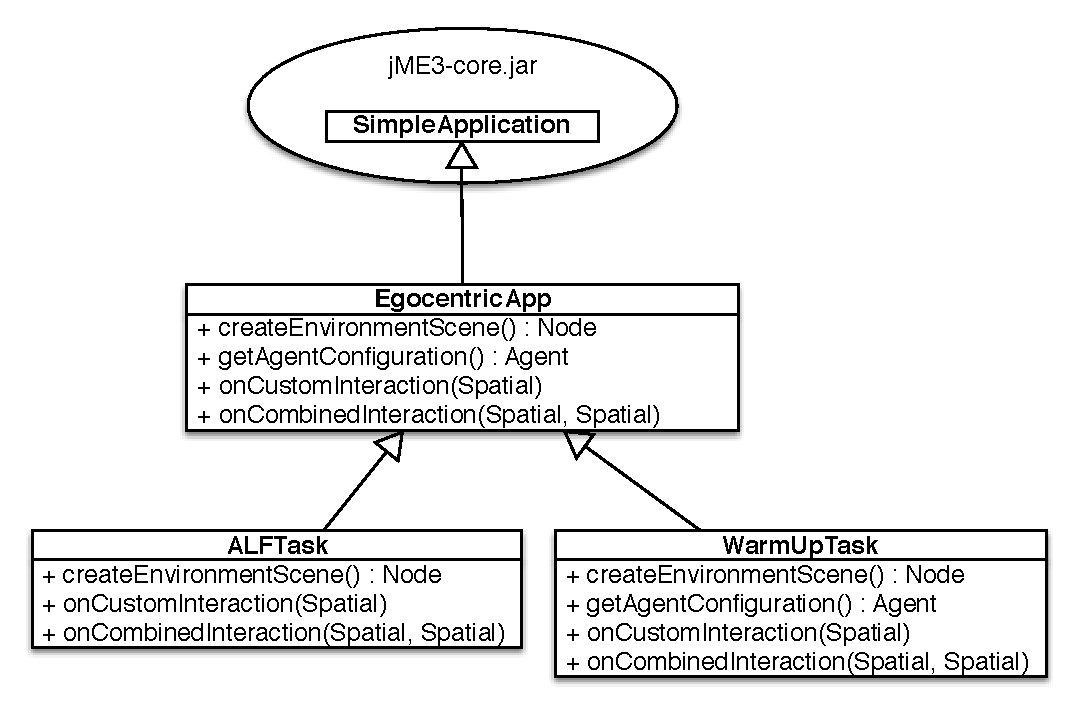
\includegraphics[width=\linewidth]{gfx/Chapter4/prototype_simulations}
	\caption{Prototype Simulations class diagram}
	\label{fig:impl_prototype_simulations}
\end{figure}

As it is the most popular open source 3D modelling application, we have decided to implement some of the 3D model in Blender. To learn about 3D modelling in Blender please refer to the on-line manual\footnote{\url{http://wiki.blender.org/index.php/Doc:2.6/Manual}}. JME3 supports direct import of .blend files. No intermediary formats are needed.\\

Next, we will shortly address each of the prototypes.
%************************************************
\subsection{WarmUpTask} % (fold)
\label{subsec:impl_warmup_task}
%************************************************
This simulation was used during the development of the framework to validate the ongoing work. For this simulation we have set up a 3D environment pragmatically. When the createEnvironmentScene() is called, it builds up a simple environment using standard shapes in the JME SDK and a few available models. The screenshot in Figure \ref{fig:impl_prototype1} illustrate a view over prototype one's 3D model. We have named it WarmUpTask because it was used as the first task in the evaluation process, helping the subjects of the evaluation familiar with simulator. The 3D model is made up by two tables, a sphere and a cylinder. All of them are configured with EgocentricContextData.\\

A detailed description of the scenario this simulation is involved in can be found in Section \ref{sec:eval_warmup_scenario}.
% section impl_warmup_task (end)

%************************************************
\subsection{ALFTask} % (fold)
\label{subsec:impl_alf_task}
%************************************************
The ALFTask represents the simulations used as the second evaluation task. For this simulation we have create a 3D model in Blender. The model resembles a one level home interior with kitchen, bathroom, living room and bathroom. The environment is populated with appliances and everyday physical objects and devices. Some of the objects have been configured with EgocentricContextData. A detailed description of the scenario this simulation is involved in can be found in Section \ref{sec:eval_alf_scenario}.\\

Interesting to note in the ALF simulations is that we have implemented a custom interaction action with the piano depicted in Figure \ref{fig:impl_piano}. The piano's EgocentricContextData is configured with interactionType CUSTOM. When the agent interacts with the piano it the simulation plays a series of musical notes.
\begin{figure}[H]
	\centering
	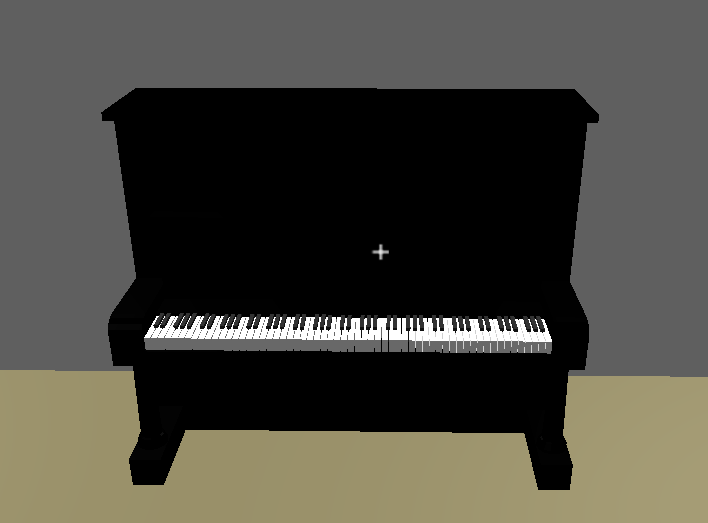
\includegraphics[width=0.8\linewidth]{gfx/Chapter4/piano}
	\caption{Example of custom interaction with the piano within the Assisted Living Facility environment}
	\label{fig:impl_piano}
\end{figure}

To implement the custom interaction behaviour, we have overridden the onCustomInteraction() method as illustrated in the following Listing. This is an example of why it is important to choose good and unique IDs for the entities while augmenting them with EgocentricContextData -- because they are used to implement business logic further on.
\begin{lstlisting}[caption={Snippet of code illustrating how to implement a CUSTOM interaction with an object},label={lst:custom_interaction}]
@Override
public void onCustomInteraction(Spatial spatial) {
    
    final EgocentricContextData data = spatial.getUserData(EgocentricContextData.TAG);
    if ("Piano".equals(data.getId())) {
        
        /* play notes */
    } else {
        super.onCustomInteraction(spatial);
    }
}
\end{lstlisting}

Moreover, we have also implemented an example of combined interaction. The screenshot from Figure \ref{fig:impl_combined_interaction}, presents an example of combined interaction when the agents tries to interact with the Cup while holding the Pot. This triggers causes the combined interaction callback to be called on the concrete simulation instance.
\begin{figure}[H]
	\centering
	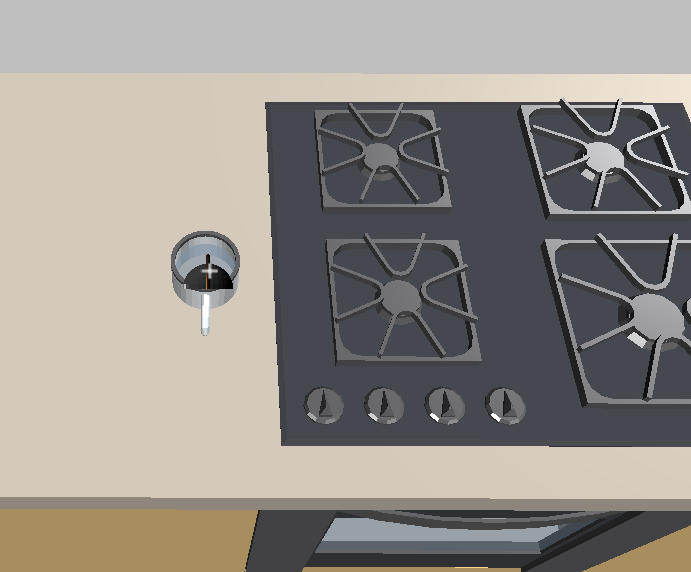
\includegraphics[width=0.8\linewidth]{gfx/Chapter4/pot_with_cup}
	\caption{Example of combined interaction within the Assisted Living Facility environment}
	\label{fig:impl_combined_interaction}
\end{figure}

To implement the combined interaction behaviour, we have overridden the onCombinedInteraction() method as illustrated in the following Listing. In this version we simply play a poring liquid sound. But, from the ALFTask we have access to all the components and assets of the simulations, so more complex actions could be taken (e.g. animating liquid pouring from the Pot into the Cup, etc).
\begin{lstlisting}[caption={Snippet of code illustrating how to implement a COMBINED interaction between two objects (when the agent acts upon an object while holding another object)},label={lst:combined_interaction}]
@Override
public void onCombinedInteraction(Spatial pickedUpObject, Spatial withObject) {
    super.onCombinedInteraction(pickedUpObject, withObject);    
    
    final EgocentricContextData data1 = pickedUpObject.getUserData(EgocentricContextData.TAG);
    final EgocentricContextData data2 = withObject.getUserData(EgocentricContextData.TAG);

    if("Pot".equals(data1.getId()) && "Cup".equals(data2.getId())) {
        /* combined interaction action */
    }
}
\end{lstlisting}
% section impl_alf_task (end)

%************************************************
\subsection{Childproof model} % (fold)
\label{subsec:impl_childproof_model}
%************************************************
For the last evaluation task we have not implemented a simulation as that is the task the subjects of the evaluation will outperform. But, in order to reduce allow them to focus on working with the framework, we have provided a 3D Blender model.\\

The model resembles a living room with a semi-integrated kitchen. The environment has been populated with appliances and everyday physical objects and devices. A detailed description of the scenario this simulation is involved in can be found in Section \ref{sec:eval_childproof_scenario}.
% section impl_childproof_model (end)

% section impl_prototype_simulations (end)